\documentclass[10pt]{article}

%%%%%%%%%%%%%%%%%%%%%%%%%%%%%%%%%%%%%%%%%%%%%%%%%%%%%%%%%%%%%%%%%%%%%%%%%%%%%%%%
% LaTeX Imports
%%%%%%%%%%%%%%%%%%%%%%%%%%%%%%%%%%%%%%%%%%%%%%%%%%%%%%%%%%%%%%%%%%%%%%%%%%%%%%%%
\usepackage{amsfonts}                                                   % Math fonts
\usepackage{amsmath}                                                    % Math formatting
\usepackage{amssymb}                                                    % Math formatting
\usepackage{amsthm}                                                     % Math Theorems
\usepackage{arydshln}                                                   % Dashed hlines
\usepackage{attachfile}                                                 % AttachFiles
\usepackage{cancel}                                                     % Cancelled math
\usepackage{caption}                                                    % Figure captioning
\usepackage{color}                                                      % Nice Colors
\input{./lib/dragon.inp}                                                % Tikz dragon curve
\usepackage[ampersand]{easylist}                                        % Easy lists
\usepackage{fancyhdr}                                                   % Fancy Header
\usepackage[T1]{fontenc}                                                % Specific font-encoding
%\usepackage[margin=1in, marginparwidth=2cm, marginparsep=2cm]{geometry} % Margins
\usepackage{graphicx}                                                   % Include images
\usepackage{hyperref}                                                   % Referencing
\usepackage[none]{hyphenat}                                             % Don't allow hyphenation
\usepackage{lipsum}                                                     % Lorem Ipsum Dummy Text
\usepackage{listings}                                                   % Code display
\usepackage{marginnote}                                                 % Notes in the margin
\usepackage{microtype}                                                  % Niceness
\usepackage{lib/minted}                                                 % Code display
\usepackage{multirow}                                                   % Multirow tables
\usepackage{pdfpages}                                                   % Include pdfs
\usepackage{pgfplots}                                                   % Create Pictures
\usepackage{rotating}                                                   % Figure rotation
\usepackage{setspace}                                                   % Allow double spacing
\usepackage{subcaption}                                                 % Figure captioning
\usepackage{tikz}                                                       % Create Pictures
\usepackage{tocloft}                                                    % List of Equations
%%%%%%%%%%%%%%%%%%%%%%%%%%%%%%%%%%%%%%%%%%%%%%%%%%%%%%%%%%%%%%%%%%%%%%%%%%%%%%%%
% Package Setup
%%%%%%%%%%%%%%%%%%%%%%%%%%%%%%%%%%%%%%%%%%%%%%%%%%%%%%%%%%%%%%%%%%%%%%%%%%%%%%%%
\hypersetup{%                                                           % Setup linking
    colorlinks=true,
    linkcolor=black,
    citecolor=black,
    filecolor=black,
    urlcolor=black,
}
\RequirePackage[l2tabu, orthodox]{nag}                                  % Nag about bad syntax
\renewcommand*\thesection{\arabic{section} }                             % Reset numbering
\renewcommand{\theFancyVerbLine}{ {\arabic{FancyVerbLine} } }              % Needed for code display
\renewcommand{\footrulewidth}{0.4pt}                                    % Footer hline
\setcounter{secnumdepth}{3}                                             % Include subsubsections in numbering
\setcounter{tocdepth}{3}                                                % Include subsubsections in toc
%%%%%%%%%%%%%%%%%%%%%%%%%%%%%%%%%%%%%%%%%%%%%%%%%%%%%%%%%%%%%%%%%%%%%%%%%%%%%%%%
% Custom commands
%%%%%%%%%%%%%%%%%%%%%%%%%%%%%%%%%%%%%%%%%%%%%%%%%%%%%%%%%%%%%%%%%%%%%%%%%%%%%%%%
\newcommand{\nvec}[1]{\left\langle #1 \right\rangle}                    %  Easy to use vector
\newcommand{\ma}[0]{\mathbf{A} }                                         %  Easy to use vector
\newcommand{\mb}[0]{\mathbf{B} }                                         %  Easy to use vector
\newcommand{\abs}[1]{\left\lvert #1 \right\rvert}                       %  Easy to use abs
\newcommand{\pren}[1]{\left( #1 \right)}                                %  Big parens
\let\oldvec\vec
\renewcommand{\vec}[1]{\oldvec{\mathbf{#1} } }                            %  Vector Styling
\newtheorem{thm}{Theorem}                                               %  Define the theorem name
\newtheorem{definition}{Definition}                                     %  Define the definition name
\definecolor{bg}{rgb}{0.95,0.95,0.95}
\newcommand{\java}[4]{\vspace{10pt}\inputminted[firstline=#2,
                                 lastline=#3,
                                 firstnumber=#2,
                                 gobble=#4,
                                 frame=single,
                                 label=#1,
                                 bgcolor=bg,
                                 linenos]{java}{#1} }
\newcommand{\python}[4]{\vspace{10pt}\inputminted[firstline=#2,
                                 lastline=#3,
                                 firstnumber=#2,
                                 gobble=#4,
                                 frame=single,
                                 label=#1,
                                 bgcolor=bg,
                                 linenos]{python}{#1} }
\newcommand{\js}[4]{\vspace{10pt}\inputminted[firstline=#2,
                                 lastline=#3,
                                 firstnumber=#2,
                                 gobble=#4,
                                 frame=single,
                                 label=#1,
                                 bgcolor=bg,
                                 linenos]{js}{#1} }
%%%%%%%%%%%%%%%%%%%%%%%%%%%%%%%%%%%%%%%%%%%%%%%%%%%%%%%%%%%%%%%%%%%%%%%%%%%%%%%%
% Beginning of document items - headers, title, toc, etc...
%%%%%%%%%%%%%%%%%%%%%%%%%%%%%%%%%%%%%%%%%%%%%%%%%%%%%%%%%%%%%%%%%%%%%%%%%%%%%%%%
\pagestyle{fancy}                                                       %  Establishes that the headers will be defined
\fancyhead[LE,LO]{Computer Systems Notes}                                  %  Adds header to left
\fancyhead[RE,RO]{Zoe Farmer}                                       %  Adds header to right
\cfoot{ \thepage }
\lfoot{CSCI 2400}
\rfoot{Han}
\title{Computer Systems Notes}
\author{Zoe Farmer}

%%%%%%%%%%%%%%%%%%%%%%%%%%%%%%%%%%%%%%%%%%%%%%%%%%%%%%%%%%%%%%%%%%%%%%%%%%%%%%%%
% Beginning of document items - headers, title, toc, etc...
%%%%%%%%%%%%%%%%%%%%%%%%%%%%%%%%%%%%%%%%%%%%%%%%%%%%%%%%%%%%%%%%%%%%%%%%%%%%%%%%
\pagestyle{fancy}                                                       %  Establishes that the headers will be defined
\fancyhead[LE,LO]{Homework 3}                                  %  Adds header to left
\fancyhead[RE,RO]{Zoe Farmer}                                       %  Adds header to right
\cfoot{\mlptikz[size=0.25in, text=on, textposx=0, textposy=0, textvalue=\thepage, textscale=0.75in]{applejack}}
\lfoot{APPM 3570}
\rfoot{Kleiber}
\title{Homework 3}
\date{Kleiber}
\author{Zoe Farmer - 101446930}
%%%%%%%%%%%%%%%%%%%%%%%%%%%%%%%%%%%%%%%%%%%%%%%%%%%%%%%%%%%%%%%%%%%%%%%%%%%%%%%%
% Beginning of document items - headers, title, toc, etc...
%%%%%%%%%%%%%%%%%%%%%%%%%%%%%%%%%%%%%%%%%%%%%%%%%%%%%%%%%%%%%%%%%%%%%%%%%%%%%%%%
\begin{document}

\maketitle

\begin{table}[!ht]
    \centering
    \scalebox{1.5}{%
    \begin{tabular}{|l|l|l|l||l|}
        \hline
        1 & 2 & 3 & 4 & T\\
        \hline
        & & & &\\
        \hline
    \end{tabular}
    }
\end{table}

\begin{easylist}[enumerate]
    @ From Chapter 2, p.\ 48: 12, 14, 15, 16, 19, 27, 28, 39, 54

    @@ An elementary school is offering 3 language classes: one in Spanish, one in French, and one in German. The classes are open to any of the 100 students in the school. There are 28 students in the Spanish class, 26 in the French class, and 16 in the German class. There are 12 students that are in both Spanish and French, 4 that are in both Spanish and German, and 6 that are in both French and German. In addition, there are 2 students taking all 3 classes.
    @@@ If a student is chosen randomly, what is the probability that he or she is not in any of the language classes?
    @@@@ Let $S$ be the set of students in Spanish, $F$ the set of French students, and $G$ the set of German students. If we define $C$ as the set of students taking language classes, we can determine the cardinality of $C$.

        \[ \begin{aligned}
        |E| =& |S| + |F| + |G| - |S \cap F| - |S \cap G| - |F \cap G| + |S \cap F \cap G|\\
            =& 28 + 26 + 16 - 12 - 4 - 6 + 2\\
            =& 50
        \end{aligned} \]

        If we let $E_1$ be the event the a student is taking a language class, we can determine the probabability of $E_1$.

        \[ 50/100 = 0.5 \]

        Similarly, if we let $E_2$ be the event that a student is \textit{not} in a language class we can determine the probability by $E_1$'s converse.

        \[ E_2 = 1 - E_1 = 1 - 0.5 = \boxed{0.5} \]

    @@@ If a student is chosen randomly, what is the probability that he or she is taking exactly one language class?
    @@@@ Again, we can use the inclusion exclusion principle to determine the cardinality of this set. Let $L$ be the set of students taking exactly one language class, and the other sets defined above.

        \[ \begin{aligned}
            |L| =& |S| + |F| + |G| - 2|S \cap F| - 2|S \cap G| - 2|F \cap G| + 4|S \cap F \cap G|\\
                =& 28 + 26 + 16 - 24 - 8 - 12 + 8\\
                =& 34
        \end{aligned} \]

        To turn this into a probability, we simply divide by the cardinality of the set of all students.

        \[ 34/100 = \boxed{0.34} \]

    @@@ If 2 students are chosen randomly, what is the probability that at least 1 is taking a language class?
    @@@@ Recall that $C$ is the set of all students not taking at least one language class. We've determined its cardinality, and we can now apply that information to determine the current problem. Each student (as was proven in part (A)) has a $0.5$ chance of not being in a language class. Therefore the probability of at least one student not being in a language class is

        \[ \frac{\binom{50}{2}}{\binom{100}{2}} = \frac{49}{198} \]

    Therefore we can find the probability of at least one student being in a language class

        \[ 1 - \frac{49}{198} = \boxed{\frac{149}{198}} \]

    @@ The following data were given in a study of a group of 1000 subscribers to a certain magazine: In reference to job, marital status, and education, there were 312 professionals, 470 married persons, 525 college graduates, 42 professional college graduates, 147 married college graduates, 86 married professionals, and 25 married professional college graduates. Show that the numbers reported in the study must be incorrect.\newline

    @@@ Let $P$, $M$, and $C$ denote, respectively, the set of professionals, married persons, and college graduates. Also let $S$ be the entire population. We can determine the cardinality of $S$ with the inclusion/exclusion principle.

        \[ \begin{aligned}
            |S| =& |P| + |M| + |C| - |P \cap M| - |P \cap C| - |M \cap C| + |P \cap M \cap C|\\
                =& 312 + 470 + 525 - 86 - 42 - 147 + 25\\
                =& 1058
        \end{aligned} \]

        Since the set (as is defined) has more individuals than surveyed, it must be incorrect.

    @@ If it is assumed that all $\begin{pmatrix}52\\5\end{pmatrix}$ poker hands are equally likely, what is the probability of being dealt
    @@@ a flush? (A hand is said to be a flush if all 5 cards are of the same suit.)
    @@@@ We first need to find the number of ways to choose 5 cards of all the same suit from a deck of cards.
        \[ \binom{4}{1} \binom{13}{5} = 5148\]
        We then need to determine the total number of ways 5 cards can be chosen.
        \[ \binom{52}{5} = 2598960 \]
        And to determine the probability we simply divide.
        \[ \frac{\binom{4}{1} \binom{13}{5}}{\binom{52}{5}} = \frac{33}{16660} = \boxed{0.00198079} \]
    @@@ one pair? (This occurs when the cards have denominations $a, a, b, c, d$, where $a, b, c$, and $d$ are all distinct.)
    @@@@ Again, we first need to determine which denomination we choose, and then which suits we take the cards from.
        \[ \binom{13}{1} \binom{4}{2} \]
        Now we need to pick three other cards that are distinct, being careful not to overcount ordering.
        \[ \frac{\binom{12}{1} \binom{4}{1} \binom{11}{1} \binom{4}{1} \binom{10}{1} \binom{4}{1}}{3!} = 1098240 \]
        Converting to probability
        \[ \left( \binom{13}{1} \binom{4}{2} \frac{\binom{12}{1} \binom{4}{1} \binom{11}{1} \binom{4}{1} \binom{10}{1} \binom{4}{1}}{3!} \right) \Big / \binom{52}{5} = \frac{352}{833} = \boxed{0.422569} \]

    @@@ two pairs? (This occurs when the cards have denominations $a, a, b, b, c$, where $a, b$, and $c$ are all distinct.)
    @@@@ Using a similar process, we first find our pairs, and then the other cards, being careful not to overcount.
        \[ \binom{13}{1}\binom{4}{2} \binom{12}{1} \binom{4}{2} \binom{11}{1} \binom{4}{1} \frac{1}{2!} = 123552 \]
        Dividing to find the probability we get
        \[ \boxed{0.04754} \]
    @@@ three of a kind? (This occurs when the cards have denominations $a, a, a, b, c$, where $a, b$, and $c$ are all distinct.)
    @@@@ Extending the theory, we can find our three of a kind first, and then determine the other two cards, taking care not to overcount.
        \[ \binom{13}{1} \binom{4}{3} \binom{12}{1} \binom{4}{1} \binom{11}{1} \binom{4}{1} \frac{1}{2!} = 54912 \]
        Finding the probability
        \[ \boxed{0.021128} \]
    @@@ four of a kind? (This occurs when the cards have denominations $a, a, a, a, b$.)
    @@@@ Extending the theory further, we apply the same principle.
        \[ \binom{13}{1} \binom{4}{4} \binom{12}{1} \binom{4}{1} = 624 \]
        Finding the probability
        \[ \boxed{0.00024} \]

    @@ Poker dice is played by simultaneously rolling 5 dice. Show that
    @@@ $ P\{\text{no two alike}\} = 0.0926 $
    @@@@ If we assume that poker dice is played with 6-sided dice\footnote{If we assume otherwise, then replace every 6 and 6 - $n$ with the number of faces of the dice being played with. In other words, the problem is rephrased as $\frac{\binom{n}{1} \binom{n - 1}{1} \binom{n - 2}{1} \binom{n - 3}{1} \binom{n - 4}{1}}{{\left( \binom{n}{1} \right)}^5} $ where $n$ is the number of faces.}, then we know that each die has $\binom{6}{1}$ possibilities.
        \[ \binom{6}{1} \binom{5}{1} \binom{4}{1} \binom{3}{1} \binom{2}{1} = 720\]
        Where the total number of possibilities is
        \[ \binom{6}{1} \binom{6}{1} \binom{6}{1} \binom{6}{1} \binom{6}{1} = {\left( \binom{6}{1} \right)}^5 = 7776 \]
        If we divide to find the probability, we get
        \[ \frac{\binom{6}{1} \binom{5}{1} \binom{4}{1} \binom{3}{1} \binom{2}{1}}{{\left( \binom{6}{1} \right)}^5} = \boxed{0.0925926} \]
    @@@ $ P\{\text{one pair}\} = 0.4630 $
    @@@@ Similar to the poker problem above.
        \[ \binom{6}{1} \binom{1}{1} \binom{5}{1} \binom{4}{1} \binom{3}{1} = 360 \]
        Dividing for probability
        \[ \frac{5}{108} = \boxed{0.0462963} \]
    @@@ $ P\{\text{two pair}\} = 0.2315 $
    @@@@ We now start looking at the problem in terms of slots. We first select the numbers for our two pairs, followed by the location of the first pair, the location of the second, and lastly our final number.
        \[ \binom{6}{2} \binom{5}{2} \binom{3}{2} \binom{4}{1} \]
        Converting to a probability
        \[ \frac{25}{108} = \boxed{0.231481} \]
    @@@ $ P\{\text{three alike}\} = 0.1543 $
    @@@@ Going back to the original method of identifying dice piecewise, we can determine each die face.
        \[ \binom{6}{1} \binom{1}{1} \binom{1}{1} \binom{5}{1} \binom{4}{1} \]
        Dividing to determine the probability
        \[ \frac{5}{324} = \boxed{0.0154321} \]
    @@@ $ P\{\text{full house}\} = 0.0386 $
    @@@@ A full house is when there is a triple and a pairing. We can first determine the triple, and then the pairing.
        \[ \binom{6}{1} \binom{1}{1} \binom{1}{1} \binom{5}{1} \binom{1}{1} \]
        Dividing to determine the probability
        \[ \frac{5}{1296} = \boxed{0.00385802} \]
    @@@ $ P\{\text{four alike}\} = 0.0193 $
    @@@@ The probability of this event is determined by first isolating the four alike, then identifying the fifth, and finally determining the orderings.
        \[ \binom{6}{1} \binom{5}{1} \binom{5}{1} \]
        Dividing to determine the probability
        \[ \frac{25}{1296} = \boxed{0.0192901} \]
    @@@ $ P\{\text{five alike}\} = 0.0008 $
    @@@@ Similarly to the previous problem, we need to identify the number that will be repeated, and that's it.
        \[ \binom{6}{1} \binom{1}{1} \binom{1}{1} \binom{1}{1} \binom{1}{1} \]
        Dividing to determine the probability
        \[ \frac{1}{1296} = \boxed{0.000771605} \]

    @@ Two symmetric dice have both had two of their sides painted red, two painted black, one painted yellow, and the other painted white. When this pair of dice is rolled, what is the probability that both dice land with the same color face up?
    @@@ Given the relatively small scope of the problem, we can look at each disjoint event separately.
        \[
            \underbrace{%
                \left( \frac{2}{6} \right)
                \left( \frac{2}{6} \right)
            }_{\text{Red Faces}}
            +
            \underbrace{%
            \left( \frac{2}{6} \right)
            \left( \frac{2}{6} \right)
            }_{\text{Black Faces}}
            +
            \underbrace{%
            \left( \frac{1}{6} \right)
            \left( \frac{1}{6} \right)
            }_{\text{Yellow Faces}}
            +
            \underbrace{%
            \left( \frac{1}{6} \right)
            \left( \frac{1}{6} \right)
            }_{\text{White Faces}}
            =
            \frac{5}{18}
        \]

    @@ An urn contains 3 red and 7 black balls. Players $A$ and $B$ withdraw balls from the urn consecutively until a red ball is selected. Find the probability that $A$ selects the red ball. ($A$ draws the first ball, then $B$, and so on. There is no replacement of the balls drawn.)
    @@@ Again, due to the relatively small scope of the problem we can look at each draw separately. The chance of $A$ drawing red on the first turn is $\frac{3}{10}$. On the second turn, we need $B$ to \textit{not} draw a red ball, and so the probability of this is $1 - \frac{3}{9}$. Therefore on the third turn the probability is $\left( 1 - \frac{3}{10}\right) \left(1 - \frac{3}{9} \right) \frac{3}{8}$. Continuing this progression,
        \[
            \begin{aligned}
                P_1 =& \frac{3}{10}\\
                P_3 =& \left( 1 - \frac{3}{10}\right) \left(1 - \frac{3}{9} \right) \frac{3}{8}\\
                P_5 =& \left( 1 - \frac{3}{10}\right) \left(1 - \frac{3}{9} \right) \left( 1 - \frac{3}{8} \right) \left( 1 - \frac{3}{7} \right) \frac{3}{6}\\
                P_7 =& \left( 1 - \frac{3}{10}\right) \left(1 - \frac{3}{9} \right) \left( 1 - \frac{3}{8} \right) \left( 1 - \frac{3}{7} \right) \left( 1 - \frac{3}{6}\right) \left(1 - \frac{3}{5} \right) \frac{3}{4}\\
            \end{aligned}
        \]

        If $A$ does not draw before turn 7, he will not draw a ball before $B$. In order to find the final probability, we need to sum these disjoint events, yielding

        \[ \frac{7}{12} = \boxed{0.58333} \]

    @@ An urn contains 5 red, 6 blue, and 8 green balls.  If a set of 3 balls is randomly selected, what is the probability that each of the balls will be
    @@@ of the same color?
    @@@@ We can look at the disjoint events again divided by the total number of possibilities.
        \[ \left( \binom{5}{3} + \binom{6}{3} + \binom{8}{3}\right) \Big / \binom{19}{3} = \frac{86}{969} = \boxed{0.0887513} \]
    @@@ of different colors? Repeat under the assumption that whenever a ball is selected, its color is noted and it is then replaced in the urn before the next selection. This is known as sampling with replacement.
    @@@@ Looking first at the simple case of three different colors, the problem simply becomes
        \[ \left( \binom{5}{3} \binom{6}{3} \binom{8}{3} \right) \Big / \binom{19}{3} = \frac{80}{323} = \boxed{0.247678} \]
        If we assume that each ball is replaced whenever it is selected, the problem becomes much harder. We first determine the odds of drawing each ball, and then adjust for ordering.
        \[ \frac{5}{19} \cdot \frac{6}{19} \cdot \frac{8}{19} 3! = \frac{1440}{6859} = \boxed{0.209943} \]

    @@ There are 5 hotels in a certain town. If 3 people check into hotels in a day, what is the probability that they each check into a different hotel? What assumptions are you making?
    @@@ After the first individual checks into a hotel, the odds that the next person will check into a different hotel is $\frac{4}{5}$. The odds that the third person will check into a different hotel is similarly $\frac{3}{5}$. Therefore the total probability is
        \[ \frac{4}{5} \cdot \frac{3}{5} = \frac{12}{25} = \boxed{0.48} \]
        We are assuming that each hotel is equally likely to be chosen, and that all hotels are comparable in terms of service, pricing, location, etc. We are also assuming that every person is randomly picking hotels to stay in.

    @@ Compute the probability that a bridge hand is void in at least one suit.
    @@@ Let $E_i$ be the event that the bridge hand is void in a given suit, for $i=1, 2, 3, 4$. We wish to find

    \[ P(\cup^4_{i=1}E_i) = P(E_1 \cup E_2 \cup E_3 \cup E_4) = \sum^4_{i=1} P(E_i) - \sum_{i < j} P(E_i \cap E_j) + \sum_{i < j < k} P(E_i \cap E_j \cap E_k) \]

    Note, there are no terms $P(E_i \cap E_j \cap E_k \cap E_l)$ because we need to be dealt some cards.\newline

    If we fix the value of $i$, we can determine $P(E_i), P(E_i \cap E_j)$, and $P(E_i \cap E_j \cap E_k)$.

    \[ \begin{aligned}
        P(E_i) =& \frac{\binom{39}{13}}{\binom{52}{13}} = \frac{17063919}{1334062100} &=& 0.0127909\\
        P(E_i \cap E_j) =& \frac{\binom{26}{13}}{\binom{52}{13}} = \frac{19}{1160054} &=& 0.0000163785\\
        P(E_i \cap E_j \cap E_k) =& \frac{\binom{13}{13}}{\binom{52}{13}} = \frac{1}{635013559600} &=& 1.57477 \times 10^{-12}\\
    \end{aligned} \]

    We can now plug in our probabilities. Since many are the same, we can just multiply by a coefficient.

    \[ \begin{aligned}
        P(E_1 \cup E_2 \cup E_3 \cup E_4) &=& 4 P(E_i) - 3 P(E_i \cap E_j) + 4 P(E_i \cap E_j \cap E_k)\\
        P(E_1 \cup E_2 \cup E_3 \cup E_4) &=& 4 (0.0127909) - 3 (0.0000163785) + 4 (1.57477 \times 10^{-12})\\
                                          &=& \boxed{0.0511147}
    \end{aligned} \]

    @ A certain system can experience three different types of defects. Let $A_i (i = 1, 2, 3)$ denote the event that the system has a defect of type $i$. Suppose that $P(A_1 ) = 0.17, P(A_2 ) = 0.07, P(A_3 ) = 0.13, P(A_1 \cup A_2 ) = 0.18, P(A_1 \cup A_3 ) = 0.19, P(A_2 \cup A_3 ) = 0.18 \text{ and } P(A_1 \cap A_2 \cap A_3 ) = 0.01$. For each of the following events, (i) describe it with a Venn diagram, (ii) describe it with set notation and (iii) find its probability.
    @@ the system does not have a type 1 defect;
    @@@ First, we can demonstrate this event with a Venn diagram.

        \begin{figure}[!ht]
            \centering
            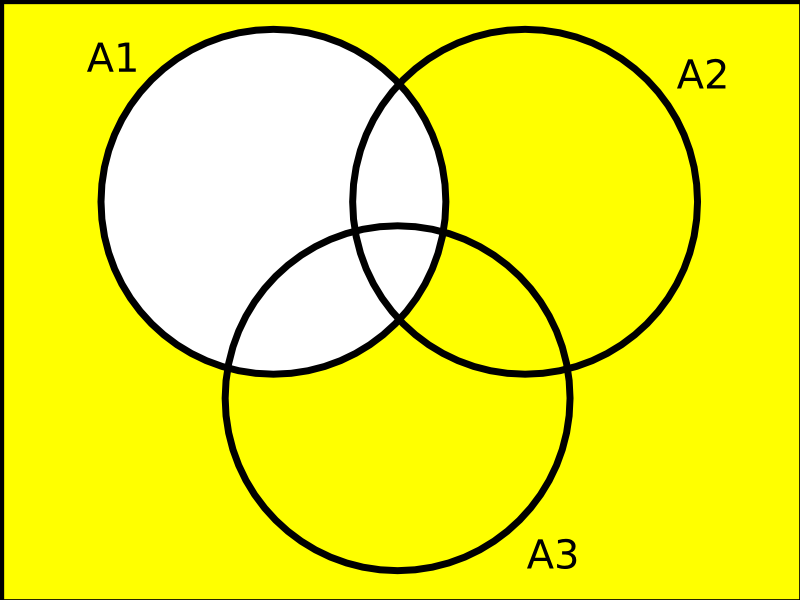
\includegraphics[scale=0.3]{./img/ps3_1.png}
        \end{figure}

        Using set notation, this problem can be displayed as

        \[ |E| = |A^c_1| \]

        Lastly we can find the probability of this event occurring.

        \[ P(E) = 1 - P(A_1) = 1 - 0.17 = \boxed{0.83} \]

    @@ the system has both type 1 and type 2 defects;
    @@@ First, we can demonstrate this event with a Venn diagram.

        \begin{figure}[!ht]
            \centering
            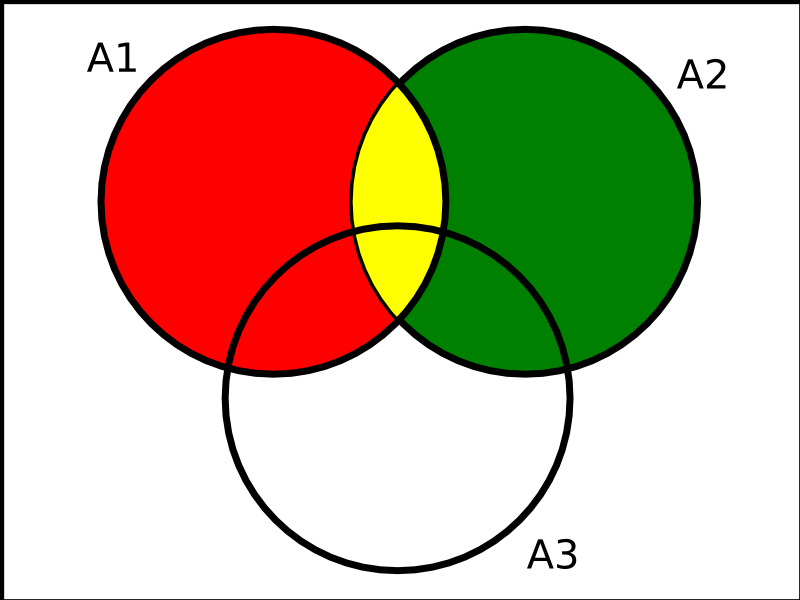
\includegraphics[scale=0.3]{./img/ps3_2.png}
        \end{figure}

        Using set notation, this problem can be displayed as

        \[ |A_1 \cap A_2| = |A_1| + |A_2| - |A_1 \cup A_2| \]

        Lastly we can find the probability of this event occurring.

        \[ P(A_1 \cap A_2) = P(A_1) + P(A_2) - P(A_1 \cup A_2) = 0.17 + 0.07 - 0.18 = \boxed{0.06} \]

    @@ the system has both type 1 and type 2 defects but not a type 3 defect;
    @@@ First, we can demonstrate this event with a Venn diagram.

        \begin{figure}[!ht]
            \centering
            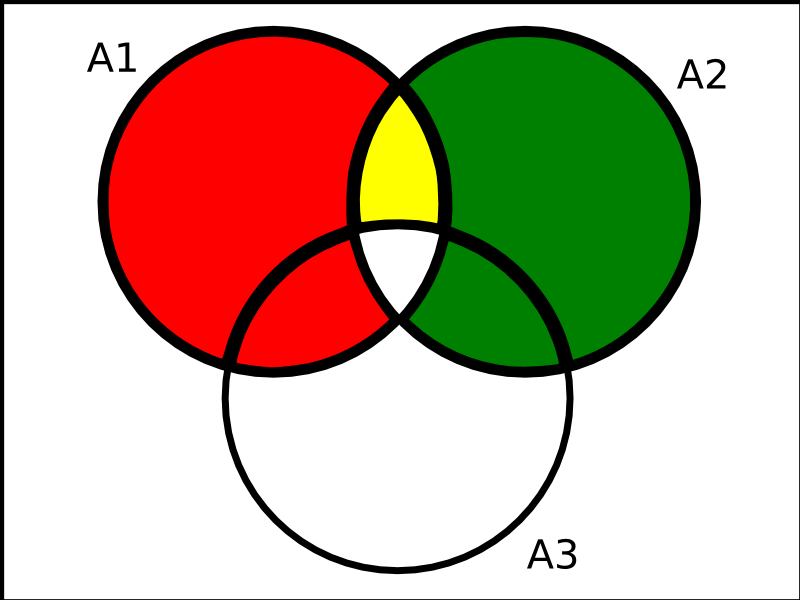
\includegraphics[scale=0.3]{./img/ps3_3.png}
        \end{figure}

        Using set notation, this problem can be displayed as

        \[ |(A_1 \cap A_2) - (A_1 \cap A_2 \cap A_3)| = |A_1| + |A_2| - |A_1 \cup A_2| - |A_1 \cap A_2 \cap A_3| \]

        Lastly we can find the probability of this event occurring.

        \[ P((A_1 \cap A_2) - (A_1 \cap A_2 \cap A_3)) = P(A_1 \cap A_2) - P(A_1 \cap A_2 \cap A_3) = 0.06 - 0.01 = \boxed{0.05} \]

    @@ the system has at most two defects.
    @@@ First, we can demonstrate this event with a Venn diagram.

        \begin{figure}[!ht]
            \centering
            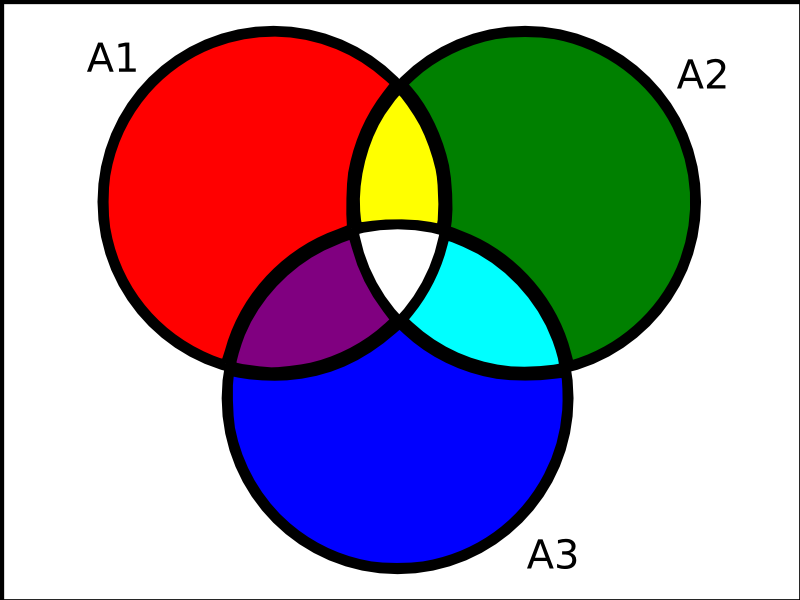
\includegraphics[scale=0.3]{./img/ps3_4.png}
        \end{figure}

        Using set notation, this problem can be displayed as

        \[ \begin{aligned}
            |(A_1 \cup A_2 \cup A_3) - (A_1 \cap A_2 \cap A_3)| =& |A_1| + |A_2| + |A_3| - |A_1 \cap A_2| - |A_1 \cap A_3| - |A_2 \cap A_3|\\
                                                                =& |A_1| + |A_2| + |A_3| - (|A_1| + |A_2| - |A_1 \cup A_2|) -\\
                                                                 & (|A_1| + |A_3| - |A_1 \cup A_3|) - (|A_2| + |A_3| - |A_2 \cup A_3|)\\
                                                                =& |A_1 \cup A_2| + |A_1 \cup A_3| + |A_2 \cup A_3| - |A_1| - |A_2| - |A_3|\\
        \end{aligned} \]

        Lastly we can find the probability of this event occurring.

        \[ \begin{aligned}
                P(E) =& P(A_1 \cup A_2) + P(A_1 \cup A_3) + P(A_2 \cup A_3) - P(A_1) - P(A_2) - P(A_3)\\
                     =& 0.18 + 0.19 + 0.18 - 0.17 - 0.07 - 0.13\\
                     =& \boxed{0.16}
            \end{aligned}
        \]

\end{easylist}

\end{document}
